%!TEX program = xelatex
% 完整编译: xelatex -> biber/bibtex -> xelatex -> xelatex
\documentclass[lang=cn,a4paper,newtx]{elegantpaper}

\title{Text-to-SQL调研报告}
\date{\zhdate{2023/2/2}}

% 本文档命令
\usepackage{array}
\usepackage{booktabs}
\usepackage{amsmath}
\usepackage{setspace}
\usepackage{array,caption}
\usepackage[labelfont=bf]{caption}
\newcommand{\ccr}[1]{\makecell{{\color{#1}\rule{1cm}{1cm}}}}
\addbibresource[location=local]{reference.bib} % 参考文献,不要删除

\begin{document}

\maketitle

\begin{abstract}
本文为对Text-to-SQL领域的一篇调研报告,从该技术的背景以及应用出发,在介绍了该领域的经典数据集后对该领域目前主流任务分为单轮任务与对话式多轮任务。后续通过该领域一些经典模型介绍这项技术近期的发展。紧接着借鉴博客推文以及自身对该领域的理解介绍了Text-to-SQL领域一些常用的方法。最后我结合本次调研做了对Text-to-SQL领域的感悟和思考。
\keywords{调研报告,Text-to-SQL}
\end{abstract}

\section{技术背景}
    \subsection{技术简介}
        自然语言被公认为是诸多领域中最便利的交互方式。但至今仍不存在一个能连接自然语言和任意领域的通用模型。对于从业者来说,无论是否精通SQL查询语言,如能通过自然语言链接关系型数据库,将会简化大量现有工作。而Text-to-SQL任务则旨在将自然语言文本转换为SQL查询语句,这项任务的提出让数据库工程师,甚至不熟悉SQL语法的使用者可以使用自然语言便捷查询数据库。
    
    \subsection{应用方向}
    \begin{enumerate}
        \item[*] \textbf{数据库查询系统},企业中通常使用众多结构化的表格存储数据,在引入Text-to-SQL技术后,普通的业务或财务人员不需要学习SQL即可直接通过自然语言于数据库交互,得到查询结果。例如企业数据库报表查询系统。
        \item[*]  \textbf{问答系统/问答机器人},Text-to-SQL作为问答系统的重要模块之一,在设计结构化表格场景发挥重要作用。例如应用于车载对话系统、企业智能报表生成系统、电话客服系统等。
        \item[*]  \textbf{搜索业务},给定一个问题,通过Text-to-SQL从数据库查询相应信息后返回,再次结合自然语言生成,生成对该问题的回答。例如百度对计算类问答与企业表格问答的探索。
        \item[*]  \textbf{数据信息增强},给定一个搜索目标或实体,可以通过Text-to-SQL方法从海量数据库中得到实体相关联的信息,丰富实体内容。
    \end{enumerate}
\section{技术介绍}
    \subsection{数据集介绍}

    一些常用中英文数据集如表1所示。表中单/多领域指数据集中数据库所属领域(食品类、工业类等)。单/多轮中单轮指数据集中每条数据为一个问题一个SQL语句回答的组合,多轮数据集中每条数据为一系列联系提问以及针对每个提问的SQL回答,且提问之间具有一定上下文联系,是对话类型数据。在此详细介绍WikiSQL、Spider、SParC、CoSQL以及CHASE数据集。不同数据集的特性,可以将其分为单领域单轮、单领域多轮、多领域单轮以及多领域多轮四种数据。而近期研究基本多领域数据,单/多轮数据均有使用,后续将介绍部分具有影响力的数据集。

    \begin{table}[h] %h表示三线表在当前位置插入
        \setlength{\abovecaptionskip}{0.05cm} %设置三线表标题与第一条线间距
        \centering
        \caption{\textbf{常用Text-to-SQL数据集}} 
        %表头文本加黑,但不加黑Table 1.字样,引入包即可:\usepackage[labelfont=bf]{caption}
        \begin{tabular*}{\hsize}{@{\extracolsep{\fill}}c c c c c c} %{\hsize}使三线表自适应宽度,c表示文本居中
        \hline
        数据集 & 数据库数量 & 单/多表 & 单/多领域 & 单/多轮 & 语言\\
        \hline 
        ATIS & 1 & 单表 & 单领域 & 单轮 & 英文 \\
        WikiSQL & 26521 & 单表 & 多领域 & 单轮 & 英文 \\
        Spider & 200 & 多表 & 多领域 & 单轮 & 英文 \\
        CSpider & 166 & 多表 & 多领域 & 单轮 & 英文 \\
        SParC & 200 & 多表 & 多领域 & 多轮 & 中文 \\
        CoSQL & 200 & 多表 & 多领域 & 多轮 & 英文 \\
        CHASE & 280 & 多表 & 多领域 & 多轮 & 中文 \\
        \hline
        \end{tabular*}
    \end{table}

    \textbf{WikiSQL\cite{1}:}发表于2017年,是最早提出的大型多数据库、单表、单轮查询的Text-to-SQL数据集。WikiSQL的每个数据库只有一个table,无需考虑主键、外键的问题,因此其SQL语句较为简单,基本由一个SQL主句加上0-3个WHERE字句条件限制构成。因此使用模板将其转化为多任务分类填空的方法在此数据库上可以取得良好效果。但是实际业务多为多表查询,且SQL语句较为复杂,因此现阶段模型在该数据集上的效果参考价值不高。
    
    \textbf{Spider\cite{2}:}发表于2018年,是一个多数据库、多表、单轮查询的Text-to-SQL数据集。包含10181个问题和5683个独特的复杂SQL查询,覆盖138个领域,Spider数据集涵盖了SQL的绝大部分高级语法,贴近现实应用,相较于WikiSQL\cite{1}具有更强的实际应用性。数据根据SQL语句难度分为Easy、Meidum、Hard与Extra Hard四种难度。但测试集不公开,需要将模型在验证集上调试到最佳性能后将模型发给Spider官方,由官方进行测试,并将结果公布在Leaderborad上确保模型方法对比的公平性。该数据集在2019年被翻译成中文提出了CSpider\cite{3}数据集。
    
    \textbf{SParC\cite{4}:}发表于2019年,是一个多数据库、多表、多轮查询的Text-to-SQL数据集,基于Spider\cite{2}数据集,收集4289个问题轮次与来自138个不同领域的200个复杂数据库。作为多轮对话形式的Text-to-SQL数据集,其要求模型考虑复杂的上下文。同时,对话的引入使得数据集具有更大的语义多样性,也要求模型具有足够的泛化性能。该数据集在目前仍具极高的参考价值。
    
    \textbf{CoSQL\cite{5}:}发表于2019年,也是一个多数据库、多表、多轮查询的Text-to-SQL数据集。相较于SPraC\cite{4},该数据集使用Wizard-of-Oz\footnote{在任务型对话里面,WOZ(Wizard-of-Oz,中文译名为绿野仙踪)数据集构造方法是一种非常常见的方法。为实现人机对话的语料库,让不同人扮演机器和人,通过他们的对话为模型提供高质量预料。}的标注方式,数据集更加贴近真实应用场景,也更具挑战性。与SParC\cite{4}类似,该数据集也基于Spider,从中收集处理了四种不同难度的SQL语句。除了每轮的SQL回答,该数据集还包括:1)每轮生成CONFIRM\--{}SQL回复,阐述本次查询的结果,方便用户确定。2)在检测到用户的问题不明确时进行CLARIFY操作,与用户确定具体查询需求。

    \textbf{CHASE\cite{6}:}发表于2021年,是首个跨领域多轮Text-to-SQL中文数据集,同样也是一个多数据库、多表、多轮查询的Text-to-SQL数据集。与SParC\cite{4}和CoSQL\cite{5}类似,对同一列表的问题之间会有实体省略等交互现象同样要求模型能理解上下文关联。相比直接翻译问题、表名和列名得到的CSpider\cite{3},该模型还保证了数据库中数据均为中文。在标注的信息上除了基本的自然语言文本和SQL,该数据集还标注了:1)上下文依赖关系。2)数据库schema的连接关系,对于自然语言文本提到的表名和列名进行了标记,此部分标注与RAT-SQL\cite{11}、IGSQL\cite{12}等模型(见2.3)中对此部分的处理相同,使用该数据集可减轻模型训练压力。

    \subsection{任务介绍}
    当今的Text-to-SQL任务聚焦于跨领域数据,单轮,多轮数据集的Text-to-SQL任务共同发展。但是难度更大,当前模型评分普遍较低的对话式多轮Text-to-SQL任务在工业上的应用更具潜力,也将是未来Text-to-SQ领域的主流研究方向。
    
    对于Text-to-SQL任务,目前广泛使用的有两大评价方式:
    
    \textbf{执行准确率(execution accuracy):}计算SQL执行结果正确的数量在数据集中的比例,此方法评分可能偏高,因为存在模型生成结果与完全不同的SQL语句都查出空结果,且被判模型生成正确的情况。

    \textbf{逻辑形式准确率(logical form accuracy):}计算模型生成的SQL语句与标注SQL语句的匹配程度,此方法评分可能偏低,因为存在同一问题不同求解方法的情况。

    目前,还没有一个指标可以独立且精确地评估模型。因此,将现有的不同指标进行结合来评估是重要的解决方法。同时,评价指标也是该领域未来值得研究的工作。

    \subsection{近期发展}
        \textbf{SQLNet\cite{7}与TypeSQL\cite{8}:}分别发表于2017年和2018年,两模型是WikiSQL提出早期两个重要的baseline。两模型针对WikiSQL较为简单的SQL语句输出使用slot filling的思想引入了如图1所示的sketch,将WikiSQL中的SQL语句分为:SELECT后的聚合符号、使用的column、WHERE子句后的column、操作符OP以及VALUE。后续将SQL生成转化为对SQL模板中多个slot的填空问题,即多任务分类问题。

        \begin{figure}[h]
            \centering
            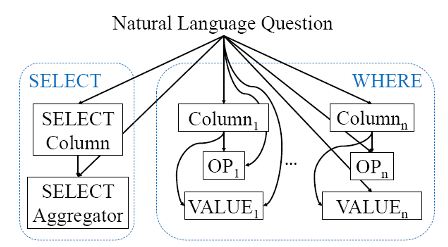
\includegraphics[width=0.7\textwidth]{sketch.png}
            \caption{基于slot filling思想的sketch模板}
        \end{figure}
        
        \textbf{TaBERT\cite{9}与GRAPPA\cite{10}:}分别发表于2020年和2021年,两模型参考BERT、RoBERTa这类自然语言预训练模型,提出了使用自然语言文本和结构化文本共同预训练的训练方式。此类预训练如GRAPPA已在\href{https://huggingface.co/Salesforce/grappa_large_jnt}{huggingface}网站发布。与主流的自然语言处理中的预训练模型相似,上述两模型对于用户输入的自然语言文本采用MLM自监督方式训练,对于结构化文本(SQL语句)与自然语言文本以及数据库表名、列名之间的关系则提出新的自监督训练方法(如GRAPPA中提出的“给定一个自然语言句子和表头,预测SQL查询中是否出现列以及触发什么操作”的SSP任务)。解码生成SQL语句部分则使用从数据集SQL数据中人工抽取出的多种模板样例(SCFG: synchronous context-free grammer)采用匹配模板后对slot的填空问题。

        \textbf{RATSQL\cite{11}:}发表于2020年,模型基于自注意机制提出了Relation-Aware Self-Attention在自注意机制QKV的计算中注入代表先前存在的关系特征(表与列之间的关系,自然语言文本与列名,表名的关系等),将编码器模型偏向于此关系。本模型使用图来描述数据库schema,如图2所示,并将编码后的自然语言文本拼接加入图的节点集,通过Name-Base Linking(最基本的于列名,表名之间的对应),Value-Based Linking(自然语言文本中指定的数值如“4”,“Mary”等列中的值),以及最后的Memory-Schema Alignment Matrix将编码后的自然语言文本加入图中的边集,从而实现自然语言文本于结构化数据(表)的对齐。后续的解码生成SQL语句则使用应用于code generation效果良好的AST(abstract syntax tree)结构,相较于使用模板插槽的方法更为灵活。

        \begin{figure}[h]
            \centering
            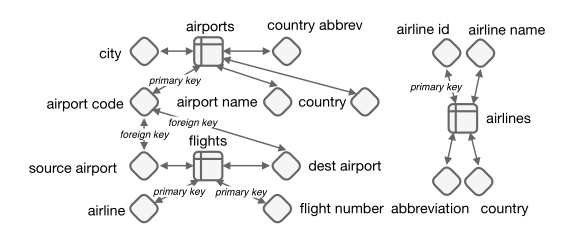
\includegraphics[width=0.8\textwidth]{graph.png}
            \caption{使用图表示数据库schema}
        \end{figure}

        \textbf{IGSQL\cite{12}:}发表于2020年,与上述针对单轮Text-to-SQL任务的工作不同,该模型针对结合对话的多轮Text-to-SQL任务改良自EditSQL\cite{13},在上下文语境理解上做出提升。模型采用BERT对自然语言文本和表名、列名进行编码,使用图表示数据库Schema(对于图的构成方式和RATSQL\cite{11}中略有不同,个人认为IGSQL的表现方式更简洁便利)。对于上下文语境的理解,除了将上一轮的输出SQL语句纳入decoder前的输入,还不断使用于自然语言文本共同经历BERT编码的表名、列名更新数据库Schema中代表的各节点之间的权重,后者也正是在EditSQL\cite{13}上做出的改进。decoder部分采用类似GPT模型的依次预测下一个token。

        总的来说近期的发展自transformer模型架构提出后Text-to-SQL任务都开始使用encoder-decoder架构以及BERT等预训练模型,在解码部分,旧一点的技术仍然使用模板填空的多分类任务,新技术则有的使用AST生成SQL,有的则参考自然语言处理中的文本生成任务(也存在其他decoder方法,这两种方法是调研中发现的较为普遍的方法)。
\section{常用方法}
    \subsection{基于模板和规则}
    早期研究多基于规则的方法。因为SQL查询语句本身是一种有很强范式的编程语言,有一定语法结构。而简单的SQL语句只涉及少数的SQL关键字和组成部分可以拆分为如图1所示的模板。针对复杂的SQL语句,可以人工设计配套的表达式匹配用户的问题和抽取SQL相应成分。这是早期基于正则表达式来识别SQL类型和抽取成分的方法。但是,正则的弊端是需要列举各种表达范式,工作量大,其次表达范式过于严格或过于宽泛均会影响准确度。随着技术的进步,后续有监督的方式被用来替代正则,如使用神经网络对问题进行编码,识别SQL类型采用分类的方法(SQLNet\cite{7}、TypeSQL\cite{8}等)

    此类方法可以快速实现一套覆盖主要问题的Text-to-SQL系统,具有较强可解释性,对定义中的SQL准确率高。但由于每类SQL都需要先定义,导致能覆盖的SQL类型较少,而完全定义所有SQL类型显然不合理,因此为了生成的SQL更灵活,样式更多,很多工作已经切换到端到端的神经网络模型。
    \subsection{基于Seq2Seq框架}
    Seq2Seq框架来自于自然语言处理中的N->M类。Text-to-SQL类似于翻译任务,与其同源的有NL-PL任务\footnote{即自然语言于编程语言之间的交互,较常见的有CodeBERT、GraphCodeBert等预训练模型}。主流的翻译模型都是基于Seq2Seq框架实现,即对输入进行编码获取语义信息,再对处理后的语义编码进行逐字解码,获取编译后的句子。典型的Seq2Seq框架并不能完全解决Text-to-SQL中面临的问题,目前主流的研究分别从编码和解码端进行改进,并取得了显著效果。
        \subsubsection{编码方法}
        \textbf{Table-aware\cite{14}},在编码器上,为充分建模问题和数据库的关系,将问题query、表名table和列名column联合,以捕捉三种隐含的关系,基本做法为将输入拼接为形如"[CLS] query [SEP] table [SEP] column1 [SEP] column2 [SEP] .... [SEP]"的长序列,将此作为输入进入编码器即可产生交互。使用该编码较为普遍。编码器可以采用典型的CNN、RNN、BERT等来学习table、column与query之间的相关性。

        \textbf{GNN编码},提出于论文Representing Schema Structure with Graph Neural Networks for Text-to-SQL Parsing\cite{15}将数据库构筑成图,利用图神经网络进行编码,以提升模型在复杂数据库schema下的表现。具体为:将表名列名各自作为节点,根据节点之间是列属于表、主键、外键建立三类边。为了能够反映每个节点与问题的相关度,模型会学习schema每个图节点向量与问题中每个词的相关度,最后问题中每个词的编码向量加上其与加权图节点编码的和,即为编码器最后输入。在涉及多表联合查询的数据集上,加入图网络可以有效增强数据库的表示,采用该方法的模型还有Global GNN\cite{16}以及再其基础上改进的RATSQL\cite{11}。

        \textbf{Relation-Aware Self-Attention},提出自RATSQL模型\cite{11}。除了使用GNN-based的编码方式外,将GNN各个节点之间的关系(schema)同时作为训练输入加入到tranformer的attention计算中,融合对齐了显式关系(schema)和隐式关系(自然语言文本和schema之间的关系),完善模型的语义提取能力(详见2.3)。

        \textbf{表格预训练},目前的语言模型如BERT无法直接对表格编码,该方法旨在将BERT像迁移至计算机视觉形成ViT一样迁移至表格数据。通过设计自监督学习任务,使模型学习如何表达用户问题以及结构化的表格之间的关系。如TaBERT模型\cite{9},后续提出的GRAPPA模型\cite{10}则在此基础上加强了用户问题、表格、sql语句三者的关系预训练(详见2.3)。
        
        \subsubsection{解码方法}
        \textbf{Pointer Network},解码端一般先生成一个token,随后再基于输入与生成的第一个token自回归地生成第二个token,以此循环直至生成停止token。本方法在此基础上改进,缩小生成token时词汇表至输入序列,如此输出能随出入改变。由于Pointer Network可以较好的满足具体数据库无关这一要求,在多领域数据集上的模型大多使用该网络。如STAMP\cite{17}、IRNet\cite{18}等模型。

        \textbf{基于强化学习},直接使用Pointer Network解码得到的where语句中多个条件之间是没有顺序的,不同的顺序实质上是等价的,但训练模型是只指定一种序列。在此使用清华学习设置奖励鼓励模型生成的SQL语句合法且正确,有效解决了单独使用Pointer Network解码的问题,模型Seq2SQL\cite{19}就是使用强化学习结合Pointer Network解码的模型。

        \textbf{基于模板},如图1所示抽象SQL语句模板,通过多分类任务向模板中筛选填充的内容,对于SQL语言形式简单的WikiSQL数据集使用该方法能达到优秀的效果。如SQLNet模型\cite{7}和与TypeSQL模型\cite{8}就是早期使用此方法生成SQL语句(详见2.3)。但是此方法对于应用场景复杂,SQL语句较为灵活的数据集则不易取得良好效果。

        \textbf{Abstract Syntax Network},传统的解码方式存在一个严重问题是生成序列中任何一个token语法有误都将导致整个sql错误。如:一开始就生成了where 这个token,那后面所有的token都是无效的,因为一开始整个输出的语法就错误了,完全无法在数据库中执行。为了解决上述问题,需要在解码过程中强制限制decoder生成的结构,使得语法合法,能有效执行。Text-to-SQL使用将logic forms转化为一棵树存储Global GNN\cite{16}、RATSQL\cite{11}都是使用的解码生成AST后再生成SQL语句。
        
    \subsection{基于阅读理解综述}
    在WikiSQL数据集上,主流模型都是采用sketch模板加填空的多分类任务的方式生成SQL,SQL Generation via Machine Reading Comprehension\cite{20}提出将该问题转化为通过多次向MRC模型提问得到回答来实现填空的动作,如图3所示。但实际上,此方法使用有较大局限性,需要SQL语句具有简单结构,在目前的业务场景中应用不佳。但按照此方法对ChatGPT进行使用,在有提供现有问题SQL模板的情况下可以具有相当好的效果。

    \begin{figure}[h]
        \centering
        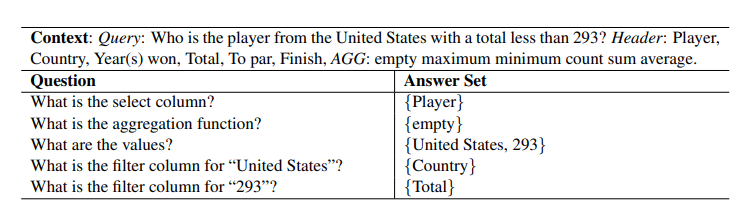
\includegraphics[width=0.9\textwidth]{MRC.png}
        \caption{论文中使用MRC实现模板填空}
    \end{figure}
    
\section{感悟与思考}
    Text-to-SQL这项技术发展至今,在单轮任务Spider数据集的\href{https://yale-lily.github.io/spider}{Leaderboard}中,当前在此领域表现较优的有CatSQL + GraPPa、Graphix-3B+PICARD和SHiP+PICARD三模型。综合考虑三模型在两评价指标下的评分发现,当前sota水平可达75$\%$左右,最新更新在2022年9月份,榜单上靠前也有12月份的模型N-best List Rerankers + PICARD可以发现此任务仍在不断发展,尚未到达瓶颈。而多轮任务的\href{https://paperswithcode.com/sota/text-to-sql-on-sparc}{SParC数据集}和\href{https://paperswithcode.com/sota/dialogue-state-tracking-on-cosql}{CoSQL数据集}榜单上除了2022年3月提出的RASAT+PICARD模型占据榜首,其余模型均早于2022年,在该任务领域sota水平中交互匹配精度为45.2$\%$,问题匹配精度为67.7$\%$,在工业应用中可能略显吃力。综合来看,在工业界应用前景更广泛的多轮Text-to-SQL任务近期研究发展不佳。下面我将阐述我对两领域的看法与认识。

    \textbf{单轮任务:}当前主流的解决问题方式集中使用Seq2Seq模式。在编码器方面,两大主流方法分别为,1)使用预训练模型解析自然语言与结构化数据之间的语义联系。2)使用图的结构保存数据库信息并将自然语言文本在图上实现融合对齐。前者更有利于后续多模态领域大一统思想的发展,后者图这个数据结构本身适合描述数据库各列、表以及自然语言文本之间的关系,在融入注意力机制后个人认为其发展潜力较大。在解码器方面,也是存在使用AST规范生成或是类似自然语言生成问题中的自回归预测两种主流方法。根据AST在NL-PL领域的效果,相信AST的方法能让模型更好地理解SQL语句的语义。
    
    \textbf{多轮任务:}我个人对多轮Text-to-SQL任务更好奇,也正是因为该任务在工业界具有更大的应用潜力。经过先前在ChatGPT中使用R语言dataTable数据列与表,以及自然语言问题生成对dataTable数据操作的R语言代码可以验证:ChatGPT在解决类似多轮Text-to-SQL任务可以表现出良好的上下文理解性以及回答的正确性。我相信学习ChatGPT模型的超大模型、超多参数的思路能使该领域在上下文联系理解以及最后的回答效果上有较大的突破。
    

    

    

\nocite{*}
% \printbibliography[heading=bibintoc, title=\ebibname]
%------------------------------------------------------------------------
\begin{thebibliography}{99}  

\bibitem{1}Zhong, V., Xiong, C. & Socher, R.Seq2SQL: Generating Structured Queries from Natural Language using Reinforcement Learning.. arXiv:1709.00103 [cs.CL]
\bibitem{2}Yu, T., Zhang, R., Yang, K., Yasunaga, M., Wang, D., Li, Z., Ma, J., Li, I., Yao, Q., Roman, S., Zhang, Z. & Radev, D.Spider: A Large-Scale Human-Labeled Dataset for Complex and Cross-Domain Semantic Parsing and Text-to-SQL Task.. arXiv:1809.08887 [cs.CL]
\bibitem{3}Min, Q., Shi, Y. & Zhang, Y.A Pilot Study for Chinese SQL Semantic Parsing.. arXiv:1909.13293 [cs.CL]
\bibitem{4}Yu, T., Zhang, R., Yasunaga, M., Tan, Y., Lin, X., Li, S., Er, H., Li, I., Pang, B., Chen, T., Ji, E., Dixit, S., Proctor, D., Shim, S., Kraft, J., Zhang, V., Xiong, C., Socher, R. & Radev, D.SParC: Cross-Domain Semantic Parsing in Context.. arXiv:1906.02285 [cs.CL]
\bibitem{5}[CoSQL: A Conversational Text-to-SQL Challenge Towards Cross-Domain Natural Language Interfaces to Databases](https://aclanthology.org/D19-1204) (Yu et al., EMNLP-IJCNLP 2019)
\bibitem{6}[Chase: A Large-Scale and Pragmatic Chinese Dataset for Cross-Database Context-Dependent Text-to-SQL](https://aclanthology.org/2021.acl-long.180) (Guo et al., ACL-IJCNLP 2021)
\bibitem{7}Xu, X., Liu, C. & Song, D.SQLNet: Generating Structured Queries From Natural Language Without Reinforcement Learning.. arXiv:1711.04436 [cs.CL]
\bibitem{8}Yu, T., Li, Z., Zhang, Z., Zhang, R. & Radev, D.TypeSQL: Knowledge-based Type-Aware Neural Text-to-SQL Generation.. arXiv:1804.09769 [cs.CL]
\bibitem{9}Yin, P., Neubig, G., Yih, W. & Riedel, S.TaBERT: Pretraining for Joint Understanding of Textual and Tabular Data.. arXiv:2005.08314 [cs.CL]
\bibitem{10}Yu, T., Wu, C., Lin, X., Wang, B., Tan, Y., Yang, X., Radev, D., Socher, R. & Xiong, C.GraPPa: Grammar-Augmented Pre-Training for Table Semantic Parsing.. arXiv:2009.13845 [cs.CL]
\bibitem{11}Wang, B., Shin, R., Liu, X., Polozov, O. & Richardson, M.RAT-SQL: Relation-Aware Schema Encoding and Linking for Text-to-SQL Parsers.. arXiv:1911.04942 [cs.CL]
\bibitem{12}Cai, Y. & Wan, X.IGSQL: Database Schema Interaction Graph Based Neural Model for Context-Dependent Text-to-SQL Generation.. arXiv:2011.05744 [cs.CL]
\bibitem{13}Zhang, R., Yu, T., Er, H., Shim, S., Xue, E., Lin, X., Shi, T., Xiong, C., Socher, R. & Radev, D.Editing-Based SQL Query Generation for Cross-Domain Context-Dependent Questions.. arXiv:1909.00786 [cs.CL]
\bibitem{14}Sun, Y., Tang, D., Duan, N., Ji, J., Cao, G., Feng, X., Qin, B., Liu, T. & Zhou, M.Semantic Parsing with Syntax- and Table-Aware SQL Generation.. arXiv:1804.08338 [cs.CL]
\bibitem{15}Bogin, B., Gardner, M. & Berant, J.Representing Schema Structure with Graph Neural Networks for Text-to-SQL Parsing.. arXiv:1905.06241 [cs.CL]
\bibitem{16}Bogin, B., Gardner, M. & Berant, J.Global Reasoning over Database Structures for Text-to-SQL Parsing.. arXiv:1908.11214 [cs.CL]
\bibitem{17}Guo, D., Sun, Y., Tang, D., Duan, N., Yin, J., Chi, H., Cao, J., Chen, P. & Zhou, M.Question Generation from SQL Queries Improves Neural Semantic Parsing.. arXiv:1808.06304 [cs.CL]
\bibitem{18}Guo, J., Zhan, Z., Gao, Y., Xiao, Y., Lou, J., Liu, T. & Zhang, D.Towards Complex Text-to-SQL in Cross-Domain Database with Intermediate Representation.. arXiv:1905.08205 [cs.CL]
\bibitem{19}Zhong, V., Xiong, C. & Socher, R.Seq2SQL: Generating Structured Queries from Natural Language using Reinforcement Learning.. arXiv:1709.00103 [cs.CL]
\bibitem{20}[SQL Generation via Machine Reading Comprehension](https://aclanthology.org/2020.coling-main.31) (Yan et al., COLING 2020)
\end{thebibliography}
%------------------------------------------------------------------------

\appendix
%\appendixpage
\addappheadtotoc

\end{document}
